\subsection{Out-of-Core Graph Analytics}
\label{sec:eval:ooc}

% Same GAPBS kernels, but with constrained memory.
% Two memory budgets: 100\% (fits in \wt{} cache) and 50\% (forces evictions).
% Competitors: GraphChi, X-Stream, GridGraph, Blaze.
% Graphs: twitter_mpi, kronecker-28 (large enough to stress memory).
%
% \project{} at 100\% memory = in-memory result from Section~\ref{sec:eval:inmem}.
% At 50\%, measure graceful degradation relative to competitors.
We compare \project{} to three out-of-core systems: GraphChi, X-Stream, and Blaze.
Each system uses a different on-disk layout to maximize sequential streaming bandwidth (except X-Stream, whose preprocessing step is the creation of a binary edge list); preprocessing time is the time to construct this layout from an edge list.
To force out-of-core behavior, we cap each container at 50\% of the graph's raw on-disk edge-list size with swap disabled. Because the layouts differ, we do not tie this budget to any single system's in-memory footprint.
All systems use 64 compute threads pinned to one NUMA socket with local
memory.
We set each system's memory knob within the budget: GraphChi's \texttt{membudget} and X-Stream's \texttt{physical\_memory} to 95\% of the limit, but \project{}'s WiredTiger buffer pool (\texttt{cache\_size}) to only 30\%.
WiredTiger relies on the OS page cache for file blocks and allocating the full budget to its own cache starves the page cache and \emph{increases} the number of disk reads.
We drop the page cache before the first (cold) trial and report the mean of four warm trials.
Iostat traces (\autoref{fig:iostat-read-bw}) show constant disk I/O, confirming steady-state out-of-core execution.

% fig:ooc-results is placed side-by-side with tab:analytics-main in evaluation.tex
On kernel execution time alone, \project{} outperforms all systems except Blaze (\autoref{fig:ooc-results}).
Blaze uses direct I/O and a lock-free scatter-gather scheme called \emph{online binning}~\cite{kim2022blaze}, in which scatter threads read edge pages and route updates (PageRank contributions, not a graph mutation) into destination-partitioned bins that gather threads consume independently, avoiding atomic contention on vertex state.
This allows Blaze to fully saturate SSD bandwidth on Kronecker graphs,
where it outperforms \project{}.
On synthetic Kronecker graphs, where over half of all vertices are isolated, Blaze's frontier-based execution skips zero-degree vertices entirely, whereas \project{} pays a per-iteration cost proportional to the total vertex count; this gap narrows on real-world graphs.
On connected components, Blaze is 9\% to 46\% faster than \project{} on all graphs except Twitter, where they are tied.
For PageRank, Blaze wins on synthetic Graph500 datasets by 31\% to 37\%, but \project{} outperforms Blaze on real-world graphs: 9\% on Twitter, 17\% on uk-2007, and 65\% on com-friendster.
If we include the time to build each system's on-disk layout, \project{} is 1.3$\times$ to 6.5$\times$ faster than any other system.

\begin{figure}
  \centering
  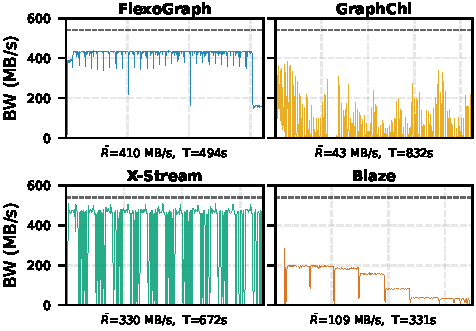
\includegraphics[width=\columnwidth]{content/fig/ooc/iostat_read_bandwidth.pdf}
  \caption{Read BW vs.\ time for PR on graph500-26. Dashed line marks 540\,MB/s device peak sequential read bandwidth. \PM{add error bars}}
  \label{fig:iostat-read-bw}
\end{figure}
\textbf{I/O bandwidth analysis.} We instrument each run with \texttt{iostat} and plot read bandwidth over time during PageRank on graph500-26.
\autoref{fig:iostat-read-bw} shows the instantaneous read bandwidth for each system, the average bandwidth, and the time taken to complete a \mbox{PageRank} run.
The dashed line marks the peak sequential bandwidth of the drive (540 MB/s).
FlexoGraph sustains the highest average read throughput of 410 MB/s (76\% of peak) with a remarkably flat profile.
WiredTiger's cursor scans produce large, sequential reads that keep the disk pipeline continuously saturated, with only brief dips at iteration boundaries.
X-Stream achieves high peak bandwidth ($\approx$480 MB/s), but exhibits a pronounced sawtooth pattern: bursts of sequential edge streaming alternate with idle periods during its gather-and-shuffle phase, pulling the average down to 330 MB/s.
Blaze begins each iteration at moderate bandwidth ($\approx$200 MB/s) that visibly decays over time, suggesting diminishing I/O as vertex values converge across iterations, yielding an average of only 109 MB/s.
Their eager elimination of inactive vertices reduces redundant I/O, so the diminishing bandwidth is not anomalous.
GraphChi fares the worst at just 43 MB/s (8\% of peak): its Parallel Sliding Windows model requires fine-grained random accesses to update vertices across shard boundaries, causing the disk to spend most of its time seeking rather than streaming.
All four systems share the same storage device, yet their bandwidth utilization spans an order of magnitude.
This gap stems not from hardware but from how each system organizes its I/O.
\project{}'s storage-engine-based design avoids both the start-stop overhead of explicit scatter-gather (X-Stream) and the random-access penalty of shard-based updates (GraphChi).
